
\documentclass[12pt,french]{article}

\usepackage[utf8]{inputenc}
\usepackage[T1]{fontenc}
\usepackage{lmodern}
\usepackage[a4paper]{geometry}
\geometry{hmargin=2.5cm,vmargin=2.5cm}
\usepackage{amsmath, amssymb}
\DeclareFontFamily{OMX}{lmex}{}
\DeclareFontShape{OMX}{lmex}{m}{n}{<->lmex10}{}
\usepackage[pdftex]{graphicx}
\usepackage{subfig}
\usepackage{lscape}
\usepackage{pdfpages}
\usepackage{float}
\usepackage{listings}
\usepackage{titlesec}
\usepackage[hypertexnames=false]{hyperref}
\newcommand{\HRule}{\rule{\linewidth}{0.5mm}}
\usepackage[tight]{shorttoc}
\renewcommand{\thesubsubsection}{\arabic{subsubsection}}
\titleformat{\subsubsection}{}{\thesubsubsection.}{0em}{}
\newcommand\invisiblesection[1]{%
  \refstepcounter{section}%
  \addcontentsline{toc}{section}{\protect\numberline{\thesection}#1}%
  \sectionmark{#1}}
\newcommand\invisiblesubsection[1]{%
  \refstepcounter{subsection}%
  \addcontentsline{toc}{subsection}{\protect\numberline{\thesection}#1}%
  \sectionmark{#1}}
\usepackage[english,francais]{babel} %à charger en dernier

\begin{document}

%%%%%%%%%%%%%%%%%%%
% début du rapport
\section{Introduction}

Notre projet porte sur le turtlebot2, un robot constitué du Kobuki, d'une kynect et d'un pc portable avec ubuntu, sur lequel nous devons réaliser un asservissement visuel. Ce dernier est un robot non holonome, il faudrat 2 odomètres pour déterminer son mouvement en translation et en rotation. \\

Pour ce faire, il faut corriger les erreurs de trajectoire liées à des défauts de fabrication et d'usure. Nous parlerons par la suite d'odométrie.

\section{Définition}

\subsection{Odométrie}
L’odomètrie se définie comme la détermination d’un déplacement grâce à des odomètres. Ces derniers sont des capteurs embarqués qui mesurent une distance parcourue, les plus classiques sont des ensembles électromécaniques. Ils sont composés d’une roue en contact avec le sol et d’une roue dentée ou une roue codeuse entraînée par la première roue. Une paire de faisceaux lumineux (ou infrarouge) sera coupée (ou non) en fonction de la roue codeuse. L’ordre dans lequel les faisceaux sont coupés donne le sens de la rotation, le nombre de front donne le déplacement.
Il existe des capteurs magnétiques qui, au lieu d’entraîner une roue codeuse, font tourner un aimant. Un capteur fixe mesure l’orientation du champ magnétique et en déduit le déplacement.\\
Dans notre cas, ceux sont des roues codeuses.\\

\subsection{Holonome}
Un robot holonome ou omni-directionnel est un robot qui posséde trois degrés de liberté, deux translations selon X et Y, et une rotation selon Z. \\
Il est donc capable de ce déplacer dans n'importe quelle direction, quelque soit son orientation. Pour se faire, il utilise trois roues composées de galets, placées à 120 degrés les une des autres.\\

Comme dit précédement, le turtlebot est non holonome, il n'a que deux degrés de liberté, une translation et une rotation suivant Z.\\ 


\section{Expérimentation}

\subsection{Ligne}

\subsubsection{Protocole}
Pour notre premier test, la ligne, nous avons pris des mesures en fonction de plusieurs vitesses et distances, 10 pour chaque cas.
Les vitesses choisies sont {0.1;0.5;0.7} $(m/s)$, et pour les distances {0.4;2.0} $m$.\\
Le protocole est le suivant:\\
Programmer le robot pour un cas, avec les parmètres de vitesse et distance voulus. \\
Dessiner une ligne au sol et définir la position initiale.\\
Placer le robot au point de départ, puis relever les valeurs des tic des roues droite et gauche, de la distance à $t_0$.\\
Lancer le programme, attendre la fin et relever les différentes valeurs avec le métre et le terminal.\\
Répéter le protocole 10 fois pour chacun des cas.\\

\vspace{5mm}

\subsubsection{Résultats}

Sur les graphiques suivants, vous pouvez observer les résulats de nos mesures ainsi que l'erreur associée. \\

\begin{figure}[h]
    \begin{minipage}[c]{.46\linewidth}
        \centering
        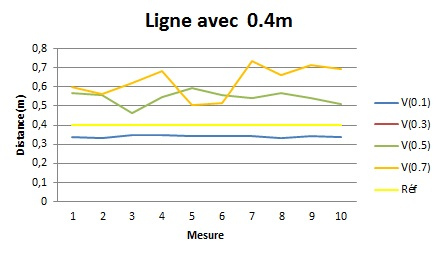
\includegraphics[width=1\textwidth]{./images/l0_4.jpg}
        \caption{Légende}
    \end{minipage}
    \hfill%
    \begin{minipage}[c]{.46\linewidth}
        \centering
        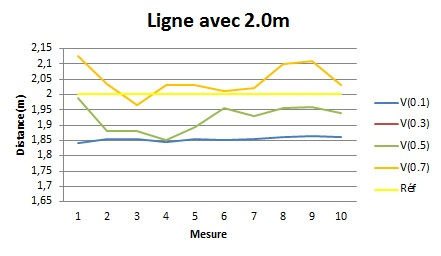
\includegraphics[width=1\textwidth]{./images/l2_0.jpg}
        \caption{Légende}
    \end{minipage}
\end{figure}

Nous remarquons que pour les vitesses basses, nous sommes toujours avec une valeur en dessous de celle attendue, tandis que pour la vitesse max nous sommes toujours au-dessus. La distance à parcourir est influencée par l'accélération et la décélération puisque nous ne les contrôlons pas, et il en suit des dérapages. Ce qui induit une grande erreur pour les petites trajectoires.\\
Nous constatons que nous tournons autour de la valeur initiale de $11,7$ $tick/mm$ pour chacun des cas, même si pour certain nous avons une grosse erreur de distance. \\
Le delta des mesures est plus petit lorsque la vitesse est proche du minimal. Nous choisissons la vistesse qui à le delta le plus faible pour que notre correction soit efficace.\\


\subsubsection{Conclusion}

Pour améliorer la précision, il faudrait gérer l'accélération et la décélération dans le but d'avoir une trajetoire plus lisse.\\
Nous trouvons les coefficients suivant:

\newpage

\subsection{Rotation}

\subsubsection{Protocole}
Pour notre second test, la ligne, nous avons pris des mesures en fonction de plusieurs vitesses angulaires et angles, 10 pour chaque cas.
Les vitesses choisies sont {0.75;1.0;1.5;3.14} $(rad/s)$, et pour les distances {pi/10;pi/4;pi} $radian$.\\
Le protocole est le suivant:\\
Programmer le robot pour un cas, avec les parmètres de vitesse angulaire et d'angle voulus.\\
Dessiner un cercle au sol ou un support troué et gradué, afin d'avoir la même surface, et définir la position initiale.\\
Placer le robot au point de départ, puis relever les valeurs des tic des roues droite et gauche, d'orientation Z et W, de l'angle à $t_0$.\\
Lancer le programme, attendre la fin et relever les différentes valeurs avec le rapporteur et le terminal.\\
Répéter le protocole 10 fois pour chaque cas.\\

\begin{figure}[h]
    \begin{minipage}[c]{.46\linewidth}
        \centering
        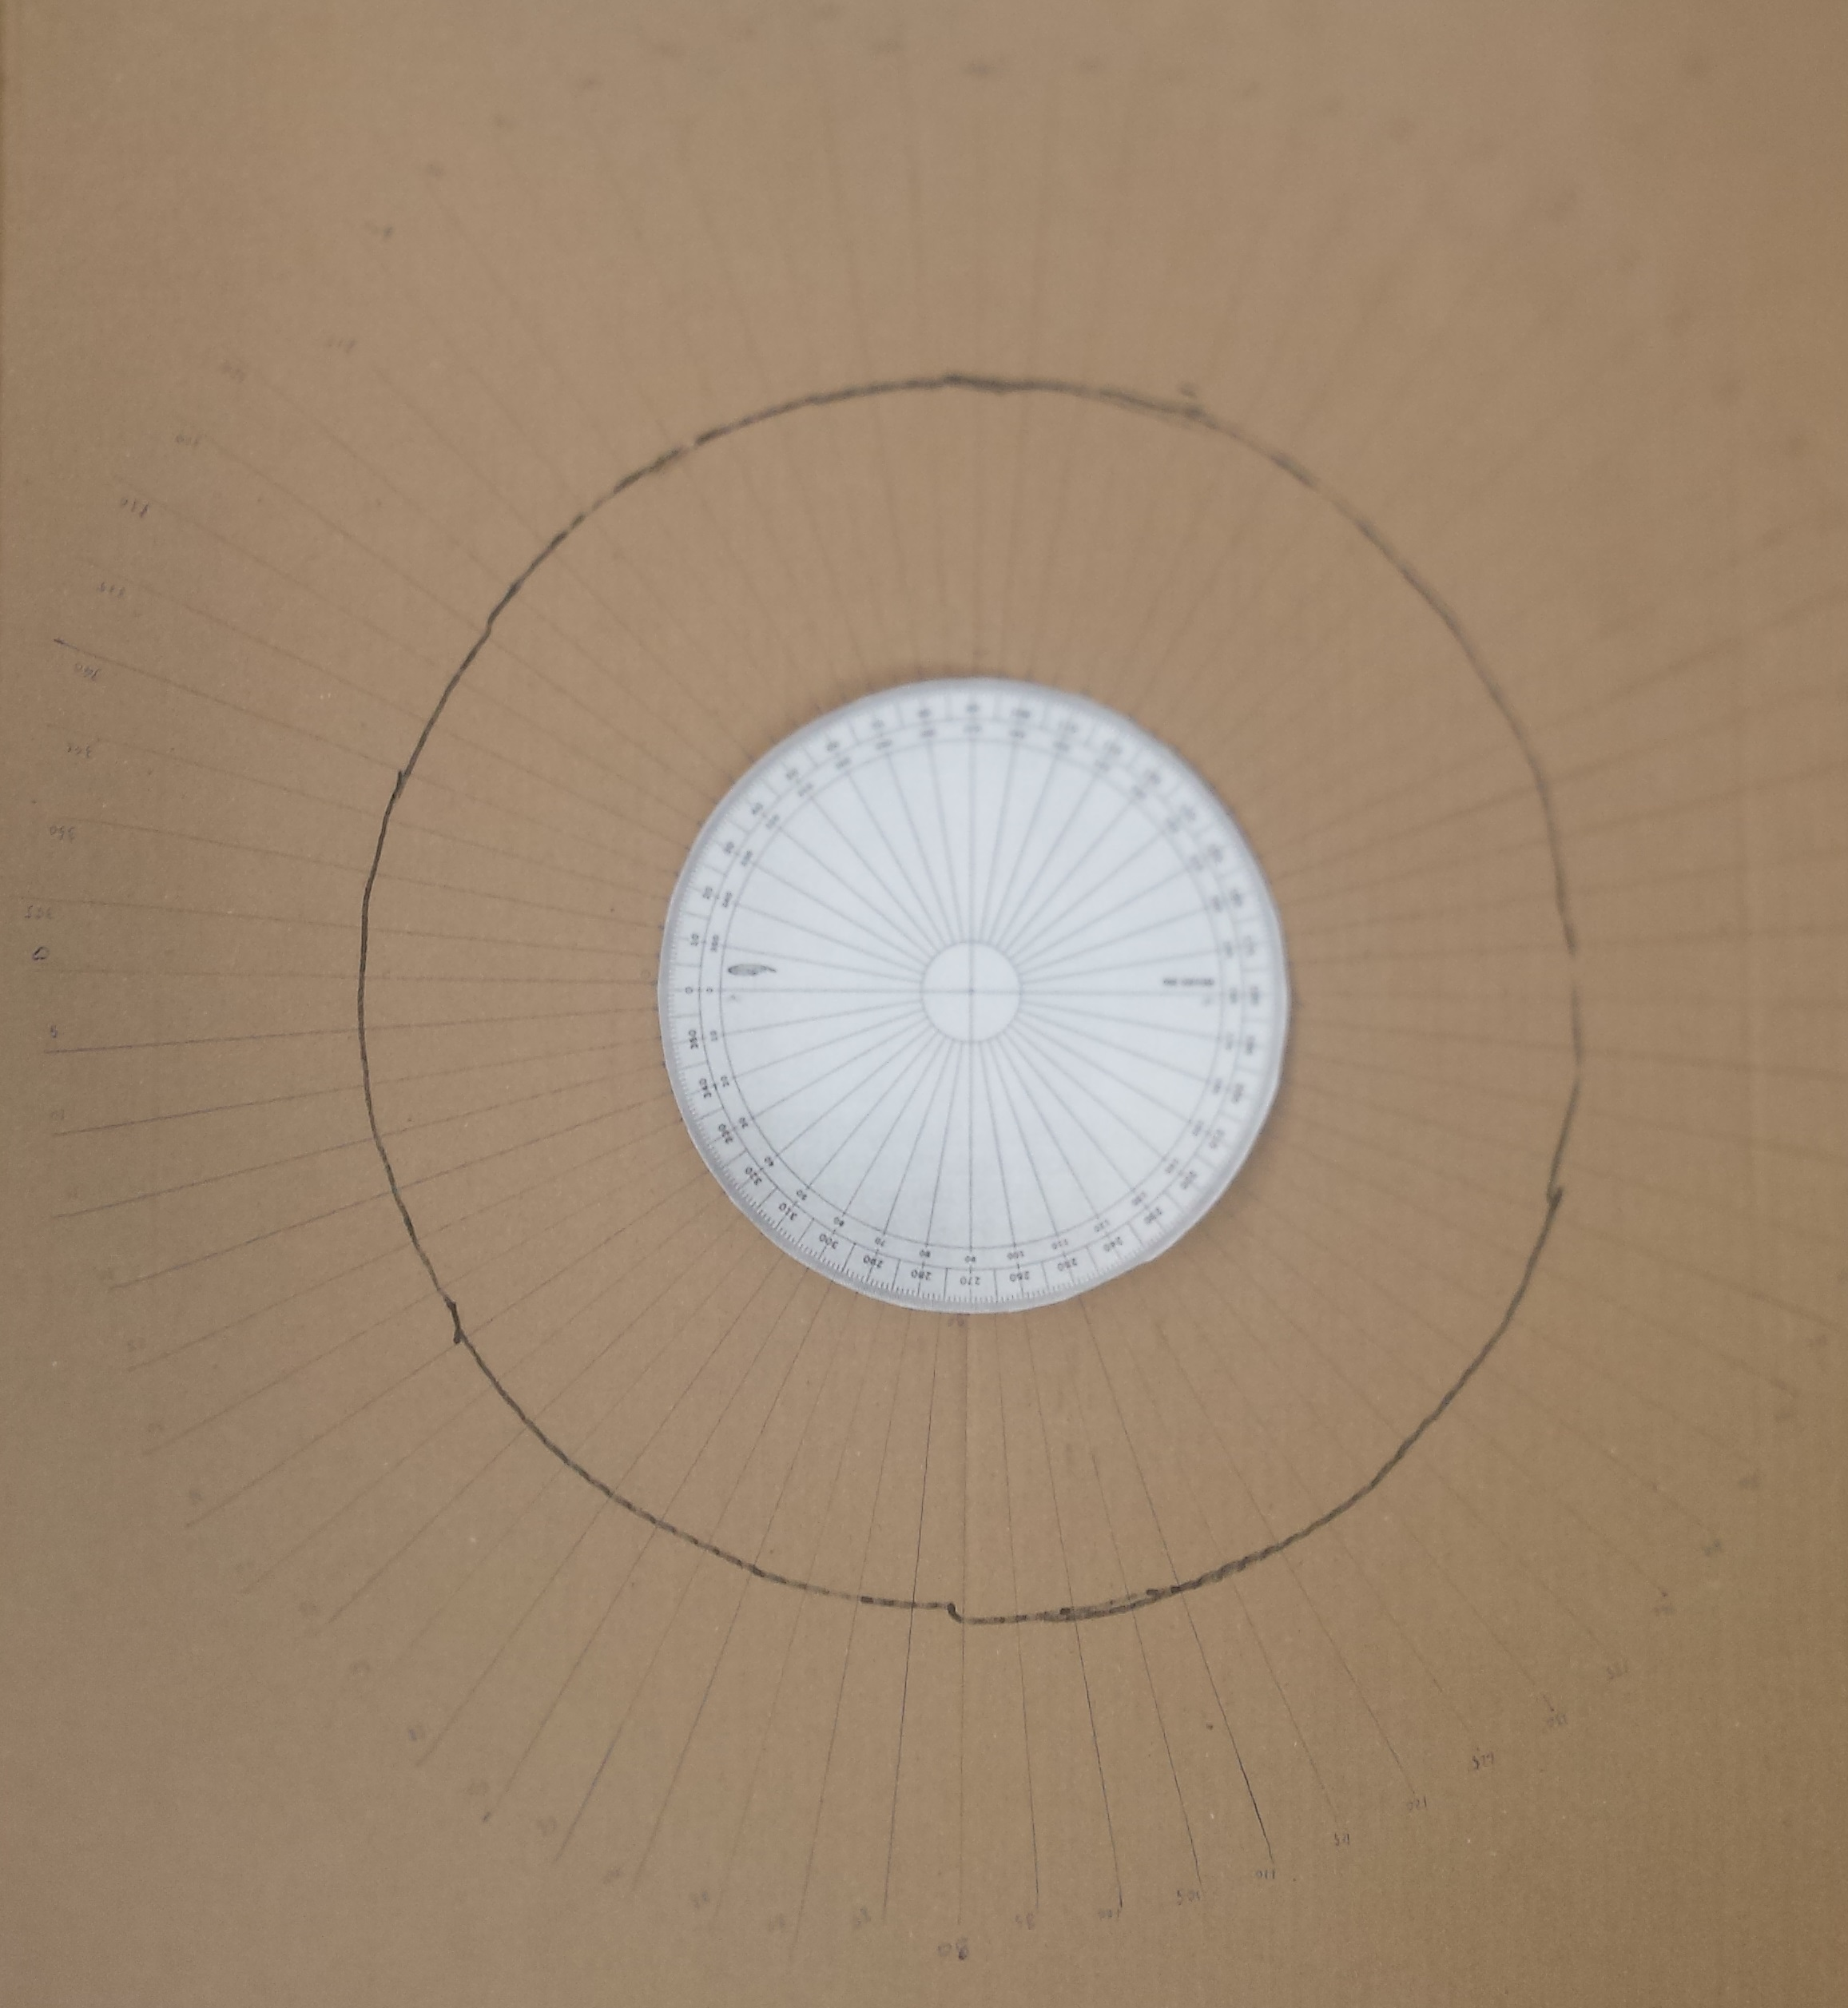
\includegraphics[width=1\textwidth]{./images/buildR.jpg}
        \caption{Rapporteur du turtlebot}
    \end{minipage}
    \hfill%
    \begin{minipage}[c]{.46\linewidth}
        \centering
        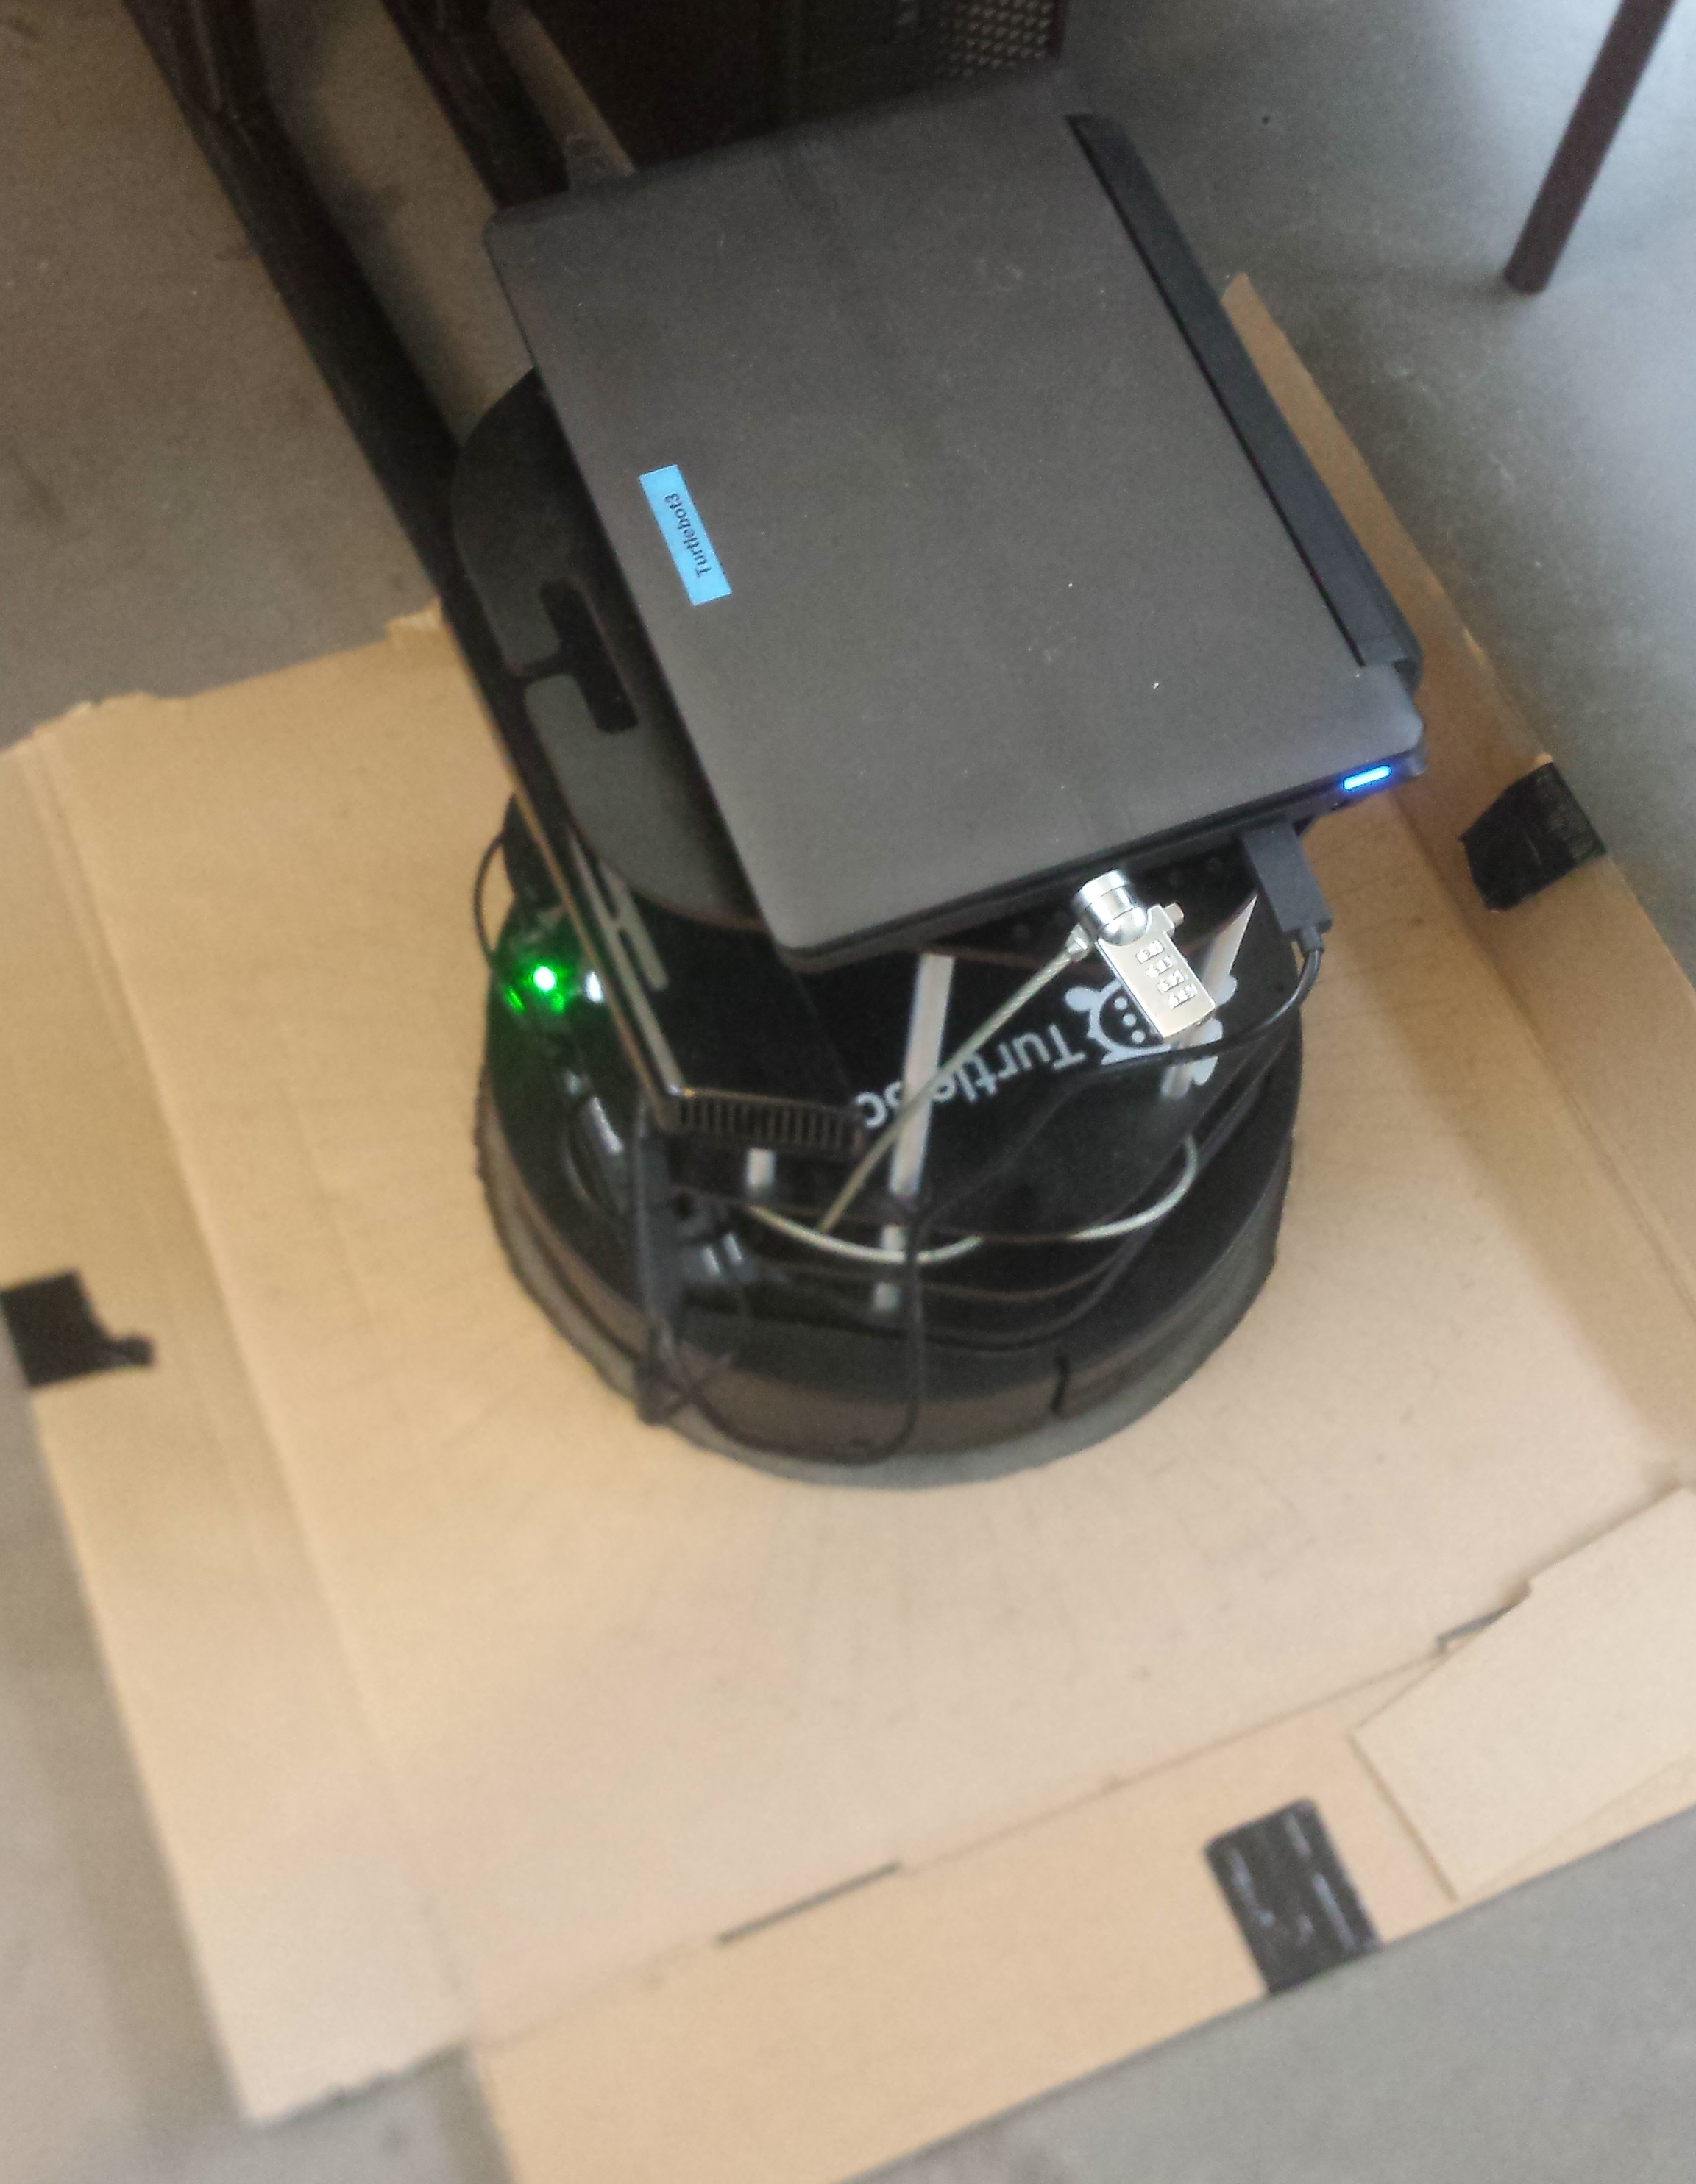
\includegraphics[width=0.8\textwidth]{./images/tr1.jpg}
        \caption{}
    \end{minipage}
\end{figure}


\subsubsection{Résultats}

Lors de l'éxpérimentation, nous constatons que le turtlebot patine aléatoirement et qu'il faut une vitesse minimale pour dépasser la force de frottement exercée par les roues libres. \\


\begin{figure}[h]
    \begin{minipage}[c]{.46\linewidth}
        \centering
        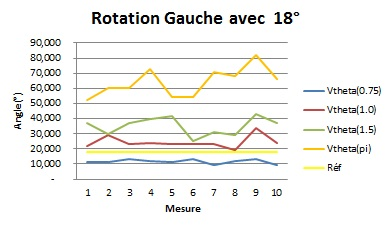
\includegraphics[width=1\textwidth]{./images/rg18.jpg}
        \caption{Légende}
    \end{minipage}
    \hfill%
    \begin{minipage}[c]{.46\linewidth}
        \centering
        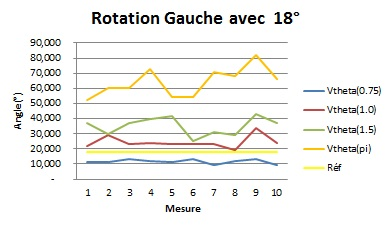
\includegraphics[width=1\textwidth]{./images/rg18.jpg}
        \caption{Légende}
    \end{minipage}
     \hfill%
    \begin{minipage}[c]{.46\linewidth}
        \centering
        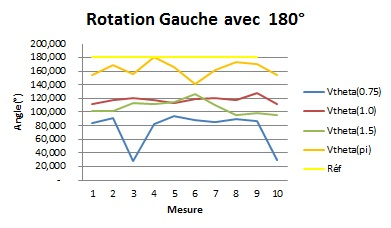
\includegraphics[width=1\textwidth]{./images/rg180.jpg}
        \caption{Légende}
    \end{minipage}
     \hfill%
    \begin{minipage}[c]{.46\linewidth}
        \centering
        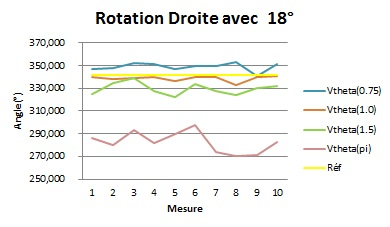
\includegraphics[width=1\textwidth]{./images/rd18.jpg}
        \caption{Légende}
    \end{minipage}
     \hfill%
    \begin{minipage}[c]{.46\linewidth}
        \centering
        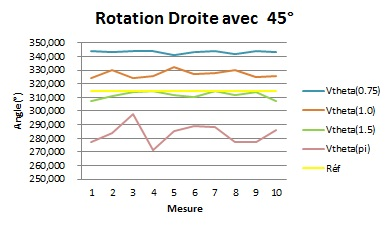
\includegraphics[width=1\textwidth]{./images/rd45.jpg}
        \caption{Légende}
    \end{minipage}
     \hfill%
    \begin{minipage}[c]{.46\linewidth}
        \centering
        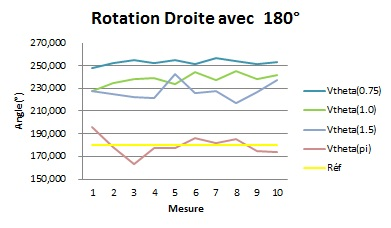
\includegraphics[width=1\textwidth]{./images/rd180.jpg}
        \caption{Légende}
    \end{minipage}
\end{figure}


A l'aide des graphiques, nous observons les variations des mesures par rapport à différente vitesse angulaire. \\
Le delta est plus petit lorsque la vitesse est proche du minimal. Nous choisissons la vistesse qui à le delta le plus faible pour que notre correction soit efficace.\\

\subsubsection{Conclusion}

Nous en concluons les coefficients et le choix des vitesses angulaires.

\end{document}




%\begin{document}
% première page
\input{./Rapport_title.tex} 



%%%%%%%%%%%%%%%%%%%
% début du rapport
\newpage
\setcounter{page}{2}


\section{Introduction}


\begin{itemize}
\item Présentation du sujet
\item Nécessité du calibrage
\end{itemize}

\section{Définition}
\subsection{Odométrie}
L’odomètrie se définie comme la détermination d’un déplacement grâce à des odomètres. Ces derniers sont des capteurs embarqués qui mesurent une distance parcourue, les plus classiques sont des ensembles électromécaniques. Ils sont composés d’une roue en contact avec le sol et d’une roue dentée ou une roue codeuse entraînée par la première roue. Une paire de faisceaux lumineux (ou infrarouge) sera coupée (ou non) en fonction de la roue codeuse. L’ordre dans lequel les faisceaux sont coupés donne le sens de la rotation, le nombre de front donne le déplacement.
Il existe des capteurs magnétiques qui, au lieu d’entraîner une roue codeuse, font tourner un aimant. Un capteur fixe mesure l’orientation du champ magnétique et en déduit le déplacement.\\

\begin{itemize}
\item Qu'est-ce?
\item L'utilité
\item Laquelle utilisée
\end{itemize}

\subsection{Robot Holonome}
La détermination du mouvement (translation et rotation) d’un robot se fait généralement grâce à 2 odomètres.
Pour les robot holonomes, dont les roues peuvent aussi glisser sur le coté, nécessitent 3 odomètres.\\

\begin{itemize}
\item Qu'est-ce?
\item Notre robot
\end{itemize}

\section{Expérimentation}
Corriger les erreurs systématiques
\subsection{Principe}
\begin{itemize}
\item Modèle(choix trajectoire)
\item Développement modèle(choix des mesures)
\item Paramètres à trouver(linéaire et angulaire)
\item Détails des calculs 
\end{itemize}
\subsection{Résultats}
\begin{itemize}
\item Analyses(courbes, tableurs)
\item Conclusion(précision, erreurs, satisfaction)
\end{itemize}

\end{document}




Le « Cahier des Charges » est le suivant :
– Notre Arduino enverra toutes les 50/100ms, le nombres de tour de la roue droite et
gauche durant ces 50/100ms. Si on utilise plusieurs capteurs de distance, on enverra
également le numéros du capteur, ainsi que la distance de l’obstacle relevée à celui-ci.
– Le Pc devra à l’aide de ces préciseuses informations recalculer la position du robot
dans la pièce. Puis localiser l’obstacle dans cette même pièce.
– Une fois les positions du Robot et de l’obstacle connues, libre à vous de l’afficher à l’écran, la stocker sur la mémoire, l’envoyer par Wifi/Bluetooth…
Dans le programme java (NetBeans) que voici, la classe « Repertoire » est une des plus importantes.\\
Sa méthode « add(DistanceGauche, DistanceDroite, NumCapteur, Distance) » va recalculer la postion du Robot, ainsi que calculer la position de l’Obstacle, pour le mettre dans un Vector.\\

Recalculer la postion du robot\\
Quand il tourne à Gauche
Place aux mathématiques !
Le déplacement du robot sera relevé tout les 50/100ms, nous pouvons donc
considère que durant ce laps de temps la trajectoire du robot est un arc de cercle, avec
I comme centre instantané de rotation. À nous de déterminer le déplacement selon X, et Y, et la rotation selon Z.
beta : $angle RS^horizon$
alpha : angle que forme le robot et l’axe des abscisses
d-alpha : angle dut au déplacement du robot durant le mouvemet
dx : deplacement selon l’axe des X durant le mouvement
dy : déplacement selon l’axe des Y durant le mouvement
Le robot tournant à gauche, l’arc de la course de la roue Droite est plus grand que
celle de la roue Gauche. En vous aidant du dessin, vous remarquez que notre
déplacement se schématise à un triange IBC, avec AD parallèle à BC.
Dans cette situation Thalès nous dit : k = AD/BC = IA/IB.
Or rappelez vous, ce déplacement à lieu sur 50/100ms. Donc dans ces conditions,
nous pouvons considèrer que l’arc AD = segement AD, de même pour BC. Notre k
n’est donc plus une inconnue !
IA = k*IB= k*(IA+AB) = k*AB/(1-k)
PS : En toute logique AB = DC = ecart entre les roues.D’où IA est connue !
Toujours là ? alors on continue ! Dans le triangle AID et sa hauteur en I
$cos(A) = AD/(2*IA)$
$A = cos^-1((AD/(2*IA)$
$d-alpha = 180 -2*A$ Nous savons de combien notre robot à tourner durant le
mouvement !
Puis dans le triangle IRS et sa hauteur en I :
$OS = IS*sin(d-alpha/2)$
$RS = 2*(IA+AB/2)*sin(d-alpha/2)$
Voilà il ne manque plus qu’une chose pour finir calculer beta !
Les calculs de beta, dx, dy
Ces calculs n’ont rien de compliqué, mais ils changent tout le temps ! En
effet d’après le dessin et uniquement dans ce cas , nous avons
$beta = A-alpha$
$dx = -RS*cos(beta)$
$dy = -RS*sin(beta)$ (dy est négatif, car le repère est celui de l’écran !!!!!! )
Nous somme dans le cas où $alpha<A$ ! De même, si le robot contiue de tourner à
gauche, le signes de dy et dx changeront !
Alors comment faire ?
En voilà une bonne question ! à nous d’observer les changements pour disséquer les
cas. Ne sachant par où commencer, j’ai divisé mes obeservations en quatres parties :
0<alpha<90, 90<alpha<180, 180<alpha<270, 270<a<360… Originale !! Puis j’ai
répertorié les changements au sein des ces parties.\\

Voici le resultat :\\
Quand il tourne à Droite
Et oui, on recommence avec la Droite. Le calcule de d-alpha et RS sont quasiment
identique, il faut juste changer les segments utilisés, car maintenant c’est l’arc Gauche
qui est plus grand que l’arc Droit.
Une fois de plus ce qui est ennuyeux, c’est de disséquer chaque cas pour les calculs de
dx, dy, beta. Mais je vous ai donné la technique plus haut, donc au boulot !
Attention : J’ai pris le sens trigo, donc quand le robot tourne à Droite d-alpha est à
soustraire de alpha !
Pour ceux qui ont l’oeil, vous remarquerez le « – » dans le calcul de dy. Rappelez vous
! Les coordonnées sont par rapport au repère de l’écran.
Le plus dur est fait, nous savons désormais placer notre robot sur une carte en
fonction des ses tours de roues. Il ne manque plus qu’à localiser l’obstacle. Ensuite je
vous parlerais du fonctionnement général du programme.
Placer l’obstacle
En résumer, nous avons la position exacte du robot et son angle, la distance de
l’obstacle par rapport au robot, et le capteur utilisé.
Dans un premier temps, nous allons situer l’obstacle en prennant le robot comme
repère.
On notera (petit) x et (petit) y pour parler des ces coordonnées par rapport au robot.
x = Distance*cos(alpha+angleCapteur)
y = distance*sin(alpha+angleCapteur)
Mais nous voulons la position par rapport à l’écran, donc on convertit.
(grand) X et (grand) Y sont ces coordonnées par rapport à l’écran.\\

